\chapter{Comparison of multi-objective evolutionary algorithms to solve the modular cell design problem} %\label{ch:conclusion}

\newcommand\HV{\mathit{HV}}
\newcommand\GD{\mathit{GD}}
\newcommand\IGD{\mathit{IGD}}

\disclose{garcia2019c}
Supplementary Material 1 is provided as an attachement.

%{{{ abstract (max ~200 words)

\section*{Abstract}
A large space of chemicals with broad industrial and consumer applications could be synthesized by engineered microbial biocatalysts. However, the current strain optimization process is prohibitively laborious and costly to produce one target chemical and often requires new engineering efforts to produce new molecules. To tackle this challenge, modular cell design based on a chassis strain that can be combined with different product synthesis pathway modules has been recently proposed.
This approach seeks to minimize unexpected failure and avoid task repetition, leading to a more robust and faster strain engineering process. In our previous study, we mathematically formulated
the modular cell design problem based on the multi-objective optimization framework. In this study, we evaluated a library of state-of-the-art multi-objective evolutionary algorithms (MOEAs) to identify the most effective method to solve the modular cell design problem.
Using the best MOEA, we found better solutions for modular cells compatible with many product synthesis modules. Furthermore, the best performing algorithm could provide better and more diverse design options that might help increase the likelihood of successful experimental implementation.
We identified key parameter configurations to overcome the difficulty associated with multi-objective optimization problems with many competing design objectives.
Interestingly, we found that MOEA performance with a real application problem, e.g., the modular strain design problem, does not always correlate with artificial benchmarks. Overall, MOEAs provide powerful tools to solve the modular cell design problem for novel biocatalysis.
%}}}
\section{Introduction}
Multi-objective optimization is a powerful mathematical toolbox widely used in engineering disciplines to solve problems with multiple conflicting design objectives \cite{coello2004}.
For example, in the field of chemical engineering, multi-objective optimization has been applied to balance design conflicts in the performance, material and energy requirements, and environmental sustainability of many different chemical processes \cite{rangaiah2009}. In industrial biotechnology, with recent advancements in synthetic biology and metabolic engineering, microorganisms can be genetically modified to produce a large space of molecules with broad applications using renewable lignocellulosic biomass or waste products as feedstocks \cite{trinh2016, lee2019}.
However, the current strain design process is prohibitively laborious and expensive for broad industrial application \cite{nielsen2016}. To overcome this challenge, recent studies have proposed the application of modular design principles commonly used in engineering \cite{bonvoisin2016} to microbial biocatalysis \cite{trinh2012, trinh2015, garcia2019, garcia2019b}.
This modular cell design approach, known as ModCell, uses multi-objective optimization to account for the competing cellular objectives when cellular metabolism is (re)designed in a modular fashion to produce a diverse class of target chemicals. ModCell has been experimentally demonstrated for biosynthesis of alcohols \cite{trinh2011, trinh2012, wilbanks2017} and esters \cite{layton2014, layton2016, layton2016b, wierzbicki2016, lee2018} in \textit{Escherichia coli}.

Despite the broad applicability of multi-objective optimization problems (MOPs) in engineering design, powerful solution algorithms remain elusive. Two approaches can be used to solve MOPs, including multi-objective evolutionary algorithms (MOEAs) and mixed integer linear programming (MILP) algorithms.
Unlike MOEA, MILP can ensure that the identified MOP solutions are optimal.
Nonetheless, MOEAs are widely used due to the following advantages over MILP: (i) computational scalability for large-scale networks by implementing efficient parallelization algorithms \cite{coello2007}, (ii) compatibility with non-linear objectives and constraints, and (iii) unbiased sampling of Pareto optimal solutions without a need to pre-specify objective preference \cite{marler2004}.
MOEAs are based on a more general type of optimization method known as evolutionary algorithms, where candidate solutions, that represent individuals of a population, are iteratively modified using heuristic rules to increase their fitness (i.e., objective function values).
Recently, much attention has been placed in the development of MOEAs to solve many-objective problems (e.g., problems with 4 or more objectives) that often correspond to real-world applications, but can be very challenging to solve with conventional MOEAs \cite{li2015}.
For the case of ModCell problem, the popular MOEA NSGAII \cite{matlabdoc, deb2001} was used to design a modular cell under 20 different production modules \cite{garcia2019}.
Due to a large space of molecules that can potentially be synthesized by modular cells, scalability issues are expected to occur when constructing modular cells that are designed to be compatible with tenths or hundreds of products.
Furthermore, using the best solver algorithm(s) allows to explore a more diverse design space, resulting in better choices for experimental implementation.

Many MOEAs have been proposed over the past two decades since the inception of landmark algorithms such as NSGAII \cite{deb2002} and SPEA2 \cite{zitzler2001}.
New MOEAs are benchmarked against libraries of artificial problems with known solutions \cite{zitzler2000, deb2002b}, and are expected to show enhanced performance for a subset of these problems in terms of scalability, identification of Pareto optimal solutions, and number of simulation generations needed to converge.
This benchmarking methodology does not always reflect MOEA performance for general problems, since specialized parameter configurations or heuristics are often used and can lead to drastically different performance towards a specific problem of interest.
Thus, the best MOEA for a certain application problem needs to be determined empirically.
In this study, we evaluated a library of state-of-the-art MOEAs to solve the multi-objective ModCell problem, with the focus on many-objectives methods.
Several cases study of increasing difficulty were examined using common performance indicators of solution optimality and diversity, and critical algorithm parameters that determine solution quality were also investigated.

%%%%%%%%%%%%%%%%%%%%%%%%%%%%%%%%%%%%%%%%%%

\section{Methods}
\subsection{Multi-objective modular cell design}
Modular cell design enables rapid generation of optimal production strains with desirable phenotypes from a modular (chassis) cell \cite{garcia2019}, requiring mimimal strain optimization cycles. These production strains are assembled from a modular cell and various compatible pathway modules. A modular cell is constructed by eliminating genes from a parent strain to maintain only core metabolic pathways shared across all pathway modules. Each module enables an optimized target product synthesis phenotype that leads to high yields, titers, and production rates. The different biochemical nature of each target metabolite can make the objectives compete with each other, turning the modular cell design problem into a multi-objective optimization problem known as ModCell2 \cite{garcia2019}:

\begin{alignat}{3}
	& \underset{ \; y_j, z_{jk}}{\max} \quad (f_1, f_2, \ldots, f_{|\mathcal{K}|})^T \quad \text{s.t.}  \label{eq4:of1} \\
	&  \quad f_k \in \, \text{arg }\underset{}{\text{max}} \Bigg\{ \frac{1}{f_k^{max}}\sum_{j \in \mathcal{J}_k} c_{jk}  v_{jk} \quad \text{s.t.} \label{eq4:of2}\\
	& \quad \qquad \sum_{j\in \mathcal{J}_k}S_{ijk}v_{jk} = 0 && \text{for all } i \in \mathcal{I}_k  \label{eq4:mb}\\
	& \quad \qquad  l_{jk} \le v_{jk} \le u_{jk}  && \text{for all } j \in \mathcal{J}_k \label{eq4:rb}\\
	& \quad \qquad  l_{jk} d_{jk} \le v_{jk} \le u_{jk} d_{jk} && \text{for all } j \in \mathcal{C} \label{eq4:db}\\
	& \quad \qquad \mathrm{where} \; d_{jk} = y_j \lor z_{jk} \; \Bigg\} && \text{for all } k \in \mathcal{K} \nonumber \\
	& \quad z_{jk}\le (1-y_j) && \text{for all } j \in \mathcal{C}, \, k \in \mathcal{K} \label{eq4:mr1}\\
	& \quad \sum_{j \in \mathcal{C}}z_{jk} \le \beta_k && \text{for all } k \in \mathcal{K} \label{eq4:mr2} \\
	& \quad \sum_{j \in \mathcal{C}} (1-y_j) \le \alpha \label{eq4:a}
\end{alignat}

\noindent where $\mathcal{I}_k$, $\mathcal{J}_k$, and $\mathcal{K}$ are the sets of metabolites, reactions, and associated production metabolic networks (i.e., the combination of the chassis organism with a specific product synthesis pathway), respectively.
The optimization problem seeks to simultaneously maximize all objectives $f_k$ \eqref{eq4:of1}.
The desirable phenotype $f_k$ for production module $k$ is determined based on key metabolic fluxes $v_{jk}$ (mmol/gDCW/h) predicted by the constraint-based metabolic model (\ref{eq4:of2}-\ref{eq4:db}) \cite{palsson2015}.
For example, the weak growth coupled to product formation (\emph{wGCP}), a common design objective, requires a high minimum product synthesis rate at the maximum growth-rate, enabling growth selection of optimal production strains. Thus, in \emph{wGCP} design, the inner optimization problem seeks to maximize growth rate while calculating the minimum product synthesis rate through the linear objective function \eqref{eq4:of2} (where {$c_{jk}$ is $1$ and $-0.0001$ for $j$ corresponding to the biomass and product reactions across all networks $k$, respectively, and 0 otherwise)
subject to: (i) mass-balance constraints \eqref{eq4:mb}, where $S_{ijk}$ represents the stoichiometric coefficient of metabolite $i$ in reaction $j$ of production network $k$, (ii) flux bound constraints \eqref{eq4:rb} that determine reaction reversibility and available substrates, where $l_{jk}$ and $u_{jk}$ are lower and upper bounds respectively, and (iii) genetic manipulation constraints \eqref{eq4:db}, i.e., deletion of a reaction $j$ in the chassis through the binary indicator $y_{j}$, or insertion of a reaction $j$ in a specific production network $k$ through the binary indicator $z_{jk}$.
The maximum product synthesis rate of each production network $k$, $f_k^{max}$, is determined by maximizing the product synthesis reaction subject to (\ref{eq4:mb}-\ref{eq4:rb}), allowing to bound $f_k$ in \textit{wGCP} between 0 and 1.
Only a subset of all metabolic reactions, $\mathcal{C}$, are considered as candidates for deletion, since many of the reactions in the metabolic model cannot be manipulated to enhance the target phenotype.
Certain reactions can be deleted in the chassis but inserted back to specific production modules, enabling the chassis to be compatible with a broader number of modules \eqref{eq4:mr1}.
The numbers of module-reaction additions and reaction deletions in the chassis are constrained by the parameters $\beta_k$ \eqref{eq4:mr2} and $\alpha$ \eqref{eq4:a}, respectively, to avoid unnecessary genetic manipulations that are generally time-consuming to implement and can lead to unforeseen phenotypes.

\subsection{Optimal solutions for a multi-objective optimization problem}
Optimal solutions for a MOP (\ref{eq4:of1}-\ref{eq4:a}) are defined based on the concept of domination: A vector $a=(a_1,\dots,a_K)^T$ \textit{dominates} another vector $b=(b_1,\dots ,b_K)^T$, denoted as  $a\prec b$ if and only if $a_i\ge b_i \; \forall i\in\{1,2,\dots,K\}$ and $a_i\ne b_i$ for at least one $i$.
Letting $x$ be the design variables (i.e., $y_j$ and $z_{jk}$) and $X$ be the feasible set determined by the problem constraints (\ref{eq4:of2}-\ref{eq4:a}), a feasible solution $x^* \in X$ of the MOP is called a Pareto optimal solution if and only if  there does not exists a vector $x'\in X$ such that $F(x')\prec F(x^*)$.
The set of all Pareto optimal solutions is called Pareto set:
\begin{equation}
\mathit{PS}:=\{x \in X:\nexists \, x' \in X, F(x') \prec F(x)\}
\end{equation}
The projection of the Pareto set in the objective space is denoted as Pareto front:
\begin{equation}
\mathit{PF}:=\{F(x): x \in PS \}
\end{equation}


\subsection{MOEA selection}
To find the best MOEAs for ModCell2, we evaluated a recent and comprehensive set of MOEAs implemented in the PlatEMO platform \cite{tian2017}.
From over 50 algorithms available in PlatEMO, we selected 2 methods for benchmark study, including NSGAII/gamultiobj and MOEAIGDNS, and 8 methods that have been specifically developed to tackle many-objective problems with discrete variables like ModCell2, including ARMOEA, EFRRR, MaOEADDFC, SPEAR, tDEA, BiGE, NSGAIII, and SPEA2SDE (Table~\ref{tab4:moeas}).
It should be noted that gamultiobj is an alternative implementation of the NSGAII algorithm available in Matlab.


\begin{table}[H]
    \caption[Summary of MOEAs]{Summary of MOEAs used in this study}
\centering
%% \tablesize{} %% You can specify the fontsize here, e.g., \tablesize{\footnotesize}. If commented out \small will be used.
%Table: MOEA summary
\rowcolors{2}{gray!25}{white}
\begin{tabular}{cm{6.5cm}m{4cm}c}
	\toprule
	Abbreviation & Name & Notes & Reference \\
	\midrule
	NSGAII & Non-dominated sorting genetic algorithm 2 & Highly applied MOEA & \cite{deb2002} \\
	gamultiobj & Matlab implementation of NSGAII &  Used in the original ModCell2 study\cite{garcia2019} & \cite{matlabdoc} \\
	MOEAIGDNS & Multi-objective evolutionary algorihtm based on an enhanced inverted generational distance metric & General MOEA with an implementation that works well with discrete variables & \cite{tian2016b} \\

	ARMOEA	& Adapation to reference points multi-objective evolutionary algorithm  & Many-objective EA based on MOEAIGDNS 	& \cite{tian2018} \\
	EFRRR	& Ensemble fitness ranking with ranking restriction	& Many-objective EA	& \cite{yuan2016a} \\
		MaOEADDFC & Many-objective evolutionary algorithm based on directional diversity and favorable convergence	& Many-objective EA	& \cite{cheng2015} \\
	SPEAR	& Strength Pareto evolutionary algorithm based on reference direction	& Many-objective EA	& \cite{jiang2017} \\
	tDEA	& $\theta$-dominance evolutionary algorithm	& Many-objective EA	& \cite{yuan2016} \\
	BiGE	& Bi-goal evolution	& Many-objective EA	& \cite{li2015a} \\
	NSGAIII & Non-dominated sorting genetic algorithm 3 	& Many-objective EA	& \cite{deb2014} \\
	SPEA2SDE & Strength Pareto evolutionary algorithm 2 with shift-based density estimation	& Many-objective EA	& \cite{li2014} \\
 \hline
\end{tabular}




    \label{tab4:moeas}
\end{table}

\subsection{Performance metrics}
To evaluate the performance of different MOEAs for a given problem, each algorithm was ran for the same number of generations, and the resulting solutions, known as Pareto front approximations, are compared using functions that measure two qualities: (i)
solution accuracy, i.e., to determine how similar the solution is to the true Pareto front and (ii) solution diversity, i.e., to evaluate how well distributed are the points in the solution.
We selected the top 5 most used  metrics according to a recent literature survey \cite{riquelme2015}.
These include, in order of popularity, hypervolume ($\HV$), generational distance ($\GD$), epsilon indicator ($\epsilon$), inverted generational distance ($\IGD$), and coverage ($C$).
Based on a recent study \cite{schutze2012}, we considered the average Hausdorff distance ($\Delta_p$), that combines $\GD$ and $\IGD$, and hence simplified the number of performance metrics to 4 in our study. These metrics are defined as follows:


$\HV$: This metric measures the volume occupied by the union of the smallest hyperboxes formed by each point in the Pareto front approximation and the reference point.  This Pareto front approximation corresponds to the solution of a specific MOEA (denoted as $\PF$) and the reference point is selected to be greater or equal to the maximum value attainable by any objective, which in our case is $\vec{1}$ (Figure~\ref{fig4:example}a):
\begin{equation}
	\HV = \bigcup\limits_{i\in I}\mathrm{Volume}(\mathrm{Box}(\PF_i,\vec{1})) \label{eq4:hv}
\end{equation}
where $I$ is the index set of $\PF$ points.

$\GD$: This metric measures the distance between the solution $\PF$ and the best Pareto front approximation determined by combining non-dominated points from all MOEA solutions of a specific case study, denoted $\PF^*$. More specifically, $\GD$ corresponds to the average Euclidean distance between each point in $\PF$ and the nearest point in $\PFs$, denoted as $d_i=\min\limits_{k \in K}\left( \sum\limits_{j \in J}(\PF_{ij} -\PFs_{kj})^2 \right)^{\frac{1}{2}}$, where $I$ ($i \in I$), $K$ ($k \in K$), and $J$ ($j \in J$) correspond to the index sets of $\PF$ points, $\PFs$ points, and problem objectives, respectively (Figure~\ref{fig4:example}b):
\begin{equation}
	 \GD = \frac{\sum\limits_{i \in I} d_i}{|I|}
\end{equation}

$\IGD$: This metric measures the distance between $\PF$ and $\PF^*$. It is determined by the average Euclidean distance between each point in $\PFs$ and the nearest point in $\PF$ denoted $\hat{d}_k=\min\limits_{i \in I}\left( \sum\limits_{j \in J}(\PFs_{kj} - \PF_{ij})^2 \right)^{\frac{1}{2}}$ (Figure~\ref{fig4:example}b):
\begin{equation}
	\IGD = \frac{\sum\limits_{k \in K} \hat{d}_k}{|K|}
\end{equation}

$\Delta_p$: This metric combines $\mathit{GD}$ and $\mathit{IGD}$ metric and thus has superior properties \cite{schutze2012}:
\begin{equation}
	 \Delta_p = \max(\mathit{GD},\mathit{IGD})
\end{equation}

$C$: This metric determines the fraction of $\PFs$ captured by the solution $\PF$ (Figure~\ref{fig4:example}c):
\begin{equation}
	C = \frac{|\PF \cap \PFs|}{|\PFs|} = \frac{|\{ k \in K : \exists i \in I \textrm{ such that } \PFs_{kj} = \PF_{ij} \textrm{ for all } j \in J \}|}{|K|}
\end{equation}

$\epsilon$: This metric is the additive epsilon indicator \cite{zitzler2002} that measures the smallest value to be added to any point in $\PF$ to make it non-dominated with respect to some point in  $\PFs$. In other words, it is the smallest value $\epsilon$ such that for any solution in $\PFs$ there is at least one solution in $\PF$ that is not worse by a difference of $\epsilon$ (Figure~\ref{fig4:example}d):
\begin{equation}
	\epsilon = \inf\{\epsilon \in \mathbb{R} : \textrm{for all }i \in I \, \exists k \in K \textrm{ such that } \PF_{ij} + \epsilon \ge \PFs_{kj} \textrm{ for all } j \in J\}
\end{equation}

Use of these metrics can be illustrated with a two-objective design example with 4 generations of improving Pareto front approximations, where the final Pareto front is used as a reference (i.e., $\PFs$) (Figure~\ref{fig4:example}e). As the Pareto fronts contain points that dominate the previous generations, all metrics decrease monotonically with the exception of $C$ that increases to a value of 1 when both Pareto front approximation and reference are the same (Figure~\ref{fig4:example}f).

\begin{figure}[H]
\centering
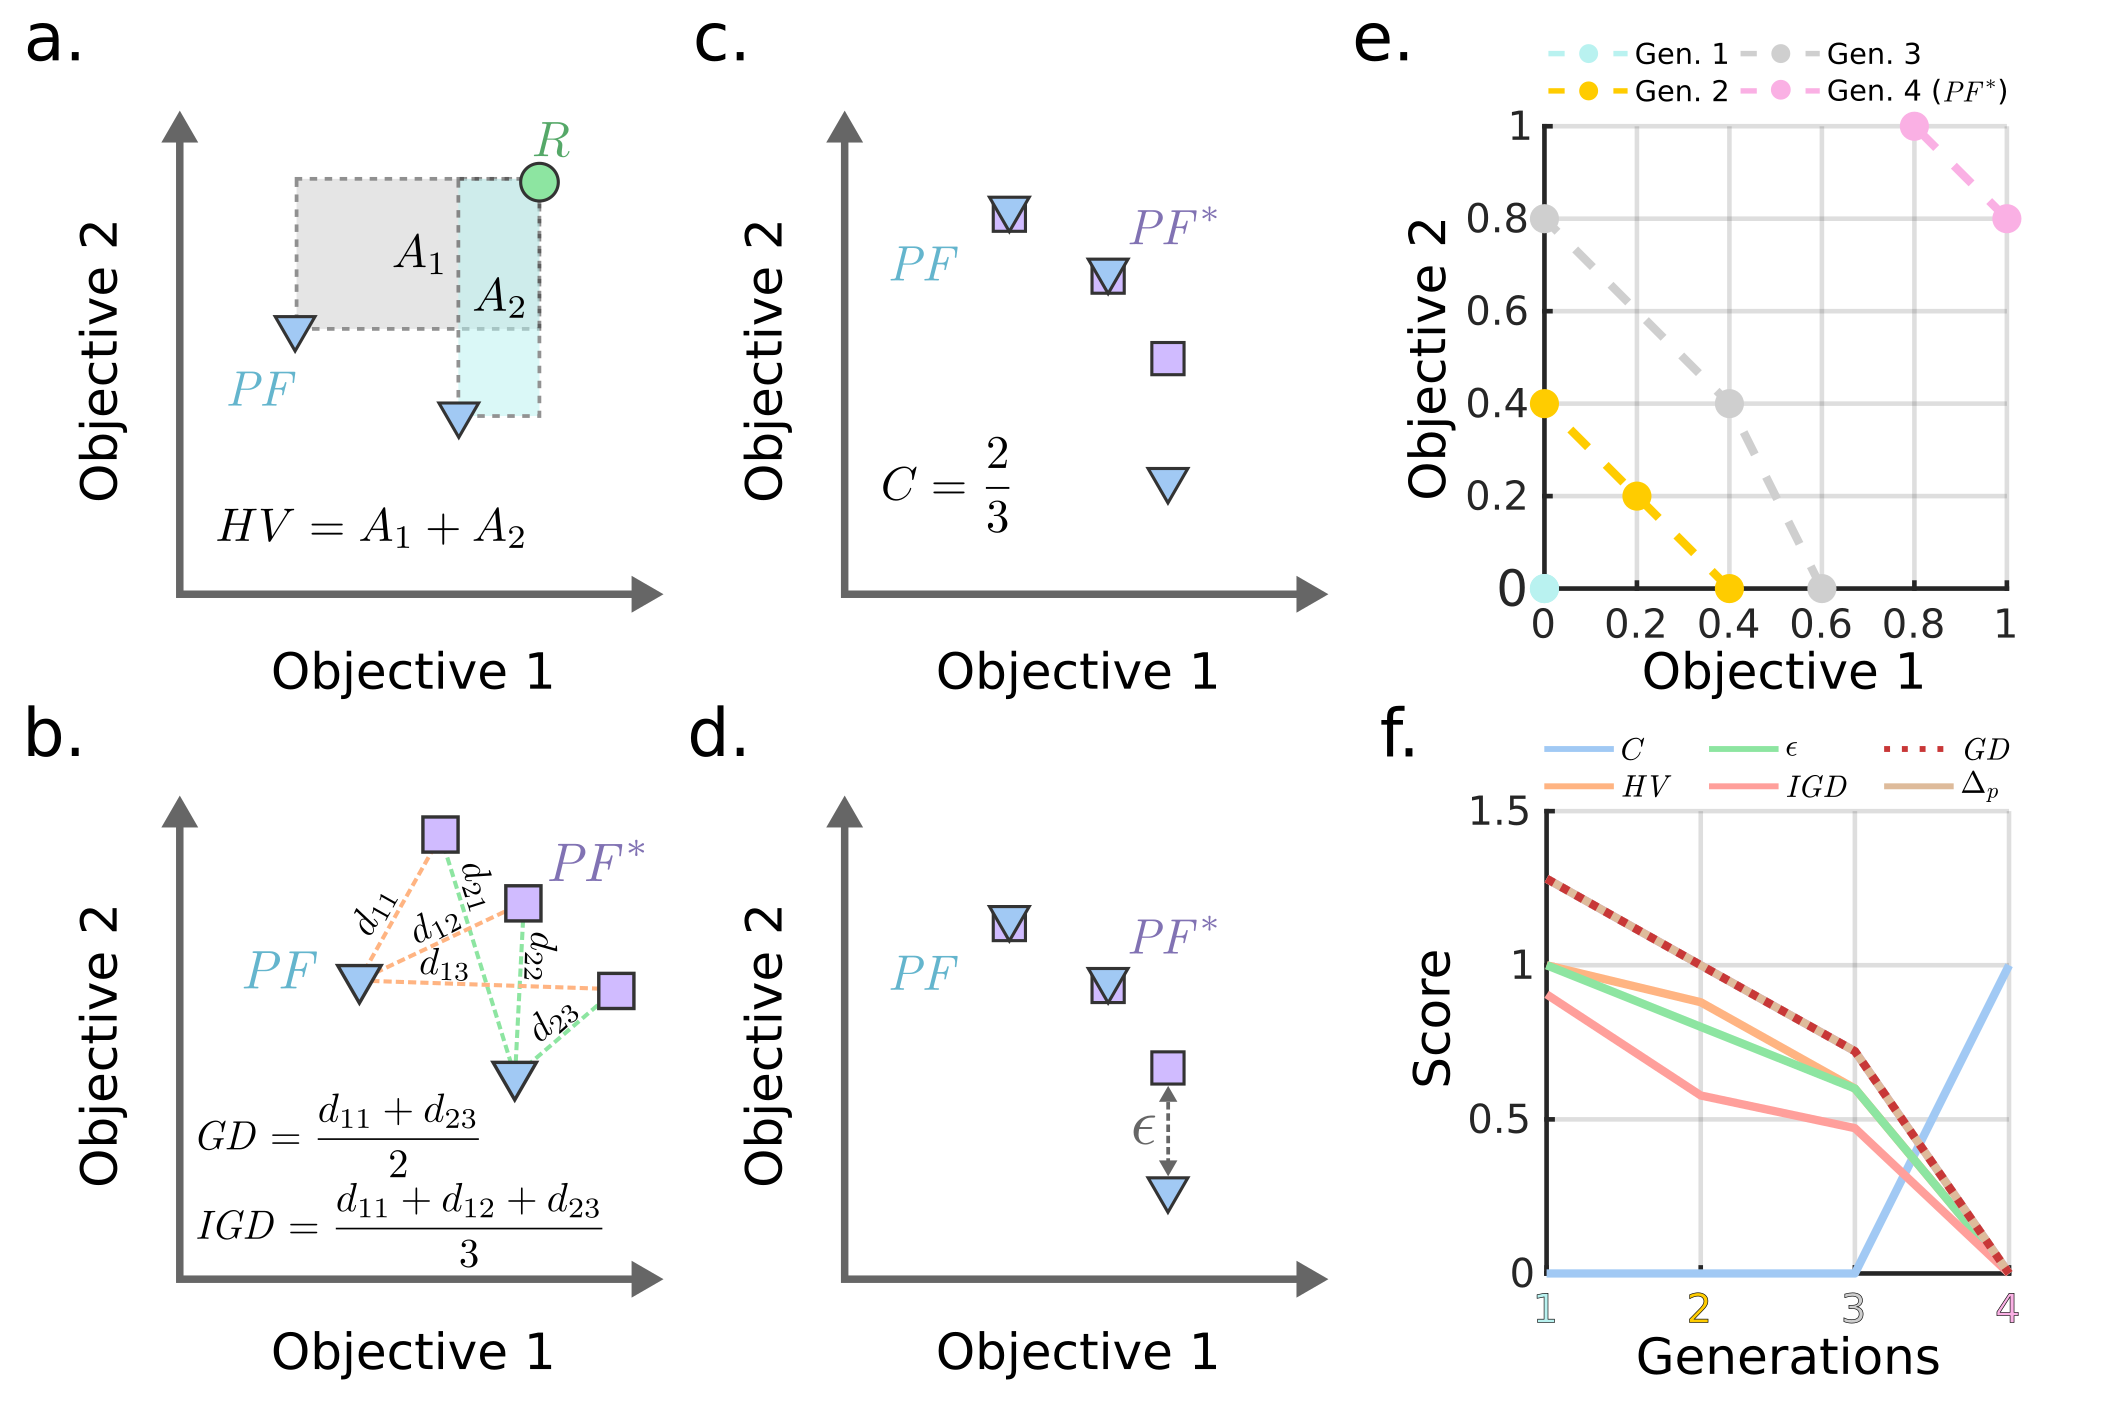
\includegraphics[width=0.8\textwidth,keepaspectratio]{example.png}
    \caption[Conceptual illustration of performance metrics]{(\textbf{a-d}) Conceptual illustration of performance metrics of MOEAs for a two-objectives design problem. $PF$ and $PF^*$ correspond to the Pareto front approximation and the best Pareto front available, respectively. The reference point $R$ must always dominate all solutions in $PF$. (\textbf{e-f}) An example of Pareto fronts with 2 dimensions and associated metrics. The 4th generation corresponds to $\PFs$ used as a reference for comparison.}
\label{fig4:example}
\end{figure}

\subsection{Algorithm parameters}
All parameters used in the simulations of this study were left as default except the following ones. The total number of generations was set to be 200, which was sufficient to reach high quality solutions for the problems of this study. In addition, the population size was set to be 100 for all algorithms unless noted otherwise.  All problems were solved in triplicates with unique random number generator seeds.

\subsection{Metabolic models}
For all simulations, we used a core \textit{E. coli} model, downloaded from the BiGG database (\url{https://bigg.ucsd.edu})  \cite{king2015}, that captures the most important metabolic pathways \cite{palsson2015}.
The product synthesis pathways for each module correspond to native \textit{E. coli} pathways together with well-characterized heterologus pathways for the synthesis of
propanol \cite{tseng2012},
butanol \cite{shen2011},
isobutanol \cite{atsumi2008},
and pentanol \cite{tseng2012}.
The metabolic reactions associated with  these pathways are described in the software implementation (Supplementary Material 1).

\subsection{Implementation} \label{sec:implementation}
The simulations were performed using the ModCell2 software framework \cite{garcia2019}.
The MOEAs are implemented in the PlatEMO Matlab library \cite{tian2017}, except \textit{gamultiobj} which is implemented as part of the Matlab Optimization Toolbox. $HV$ was calculated using the \textit{hv package} \cite{fonseca2006}. All computations were executed in a computer with the Arch Linux operative system, Intel Core i7-3770 processor, and 32 GB of random-access memory. The Matlab 2018b code used to generate the results of this manuscript is available in Supplementary Material 1 and \url{https://github.com/trinhlab/compare-moea}.

\section{Results and Discussion}
\subsection{Case 1: A 3-objectives design problem}
We first formulated a design problem that considers an \textit{E. coli} core model and 3 production modules based on the endogenous acetate, D-lactate, and ethanol biosynthesis pathways (Figure~\ref{fig4:case1}a). We used all MOEAs to solve for the problem by setting the following design parameters: \textit{wGCP} design objective, a maximum number of reaction deletions $\alpha=3$, and no module reactions $\beta=0$.
These design parameters were sufficiently restrictive to generate conflicting objectives.
A total coverage of $\PFs$ ($C=1$)  was reached within 20 generations by several algorithms (Figure~\ref{fig4:case1}b, e, h, i) and by \textit{gamultiobj} after 150 generations (Figure~\ref{fig4:case1}k), while the remaining algorithms could not attain $C$ values above 0.8 (Figure~\ref{fig4:case1}c, d, f, g, j, l). In particular, MaOEADDFC and BiGE obtained the worst $C$, $\epsilon$, and $\Delta_p$ values (Figure~\ref{fig4:case1}m).
Although $C$, $\epsilon$, and $\Delta_p$ values of BiGE indicated inferior performance, this algorithm had the lowest $HV$ since it generated only one point with a high objective value (Figure~\ref{fig4:case1}o).
Due to the simplicity of the problem, every algorithm except MaOEADDFC, tDEA, and BiGE converged to very similar Pareto fronts (Figure~\ref{fig4:case1}n-x), and 5 of them reached $C=1$, indicating convergence to the reference Pareto front (Figure~\ref{fig4:case1}y).

\subsection{Case 2: A 10-objectives design problem}
Using the same model and design parameters as in Case 1, we expanded the number of objectives to represent a more realistic scenario.
These objectives correspond to 6 endogenous pathways for biosynthesis of D-lactate, acetate, ethanol, formate, pyruvate and L-glutamate and 4 heterologous pathways for biosynthesis of propanol, butanol, isobutanol, and pentanol.
The additional objectives increased the difficulty of the problem, leading to more notable difference among algorithm performances (Figure~\ref{fig4:case2}a-k).
The SPEA2SDE algorithm displayed consistent improvement of $C$ as generations progressed, and quickly reached the smallest values of  $\epsilon$ and $\Delta_p$ (Figure~\ref{fig4:case2}h).
Other algorithms, including ARMOEA and MOEAIGDNS, also improved their $\epsilon$ values with the increasing number of generations and reached the same final values of $\epsilon$ and $\Delta_p$ as SPEA2SDE (Figure~\ref{fig4:case2}a, d). However, SPEA2SDE approached $C\cong0.6$, which is twice the value reached by the next best-performing methods (Figure~\ref{fig4:case2}l). Remarkably, SPEA2SDE outperformed every other algorithm in all metrics, except $\HV$. The $\HV$ metric continues to show bias towards algorithms that generated a small number of points and scored poorly in other metrics.


\subsection{Case 3: Use of large population size overcomes poor MOEA performance}
Increasing the number of objectives often leads to a combinatorial explosion of the number of feasible Pareto optimal points and consequently causes poor MOEA performance. This problem can be alleviated by using a larger population size to sample a broader volume of solution space \cite{ishibuchi2009}.
To test this strategy for the 10-objectives design problem above, we increased the population size from 100 to 1000 individuals while all other parameters remained unchanged.
The result showed that
ARMOEA,
MOEAIGDNS,
NSGAII,
SPEA2SDE (the best performer in Case 2),
and \textit{gamultiobj},
could reach $C$ of 0.7, $\epsilon$ of 0, and $\Delta_p$ of 0 in fewer than 50 generations (Figure~\ref{fig4:case3}a, d, g, h, j).
These 5 algorithms also yielded very similar final values across all metrics  (Figure~\ref{fig4:case3}l). The remaining algorithms converged to considerably lower $C$ values (Figure~\ref{fig4:case3}b, c, e, f, i, k).
Remarkably, NSGAII/\textit{gamultiobj}, that is not considered a many-objective solver, performed better than more recent many-objective algorithms such as NSGAIII.

One limitation of using larger populations is an increased cost in computational time. We observed that a 10-fold increase in population sizes resulted in a 10-fold increase in the run times (Figure~\ref{fig4:timing}). Nonetheless, all metrics reached a stable value in the top performing algorithms after 50 generations (out of 200 total), suggesting that fewer generations were needed by using a larger population size.  Among the best performing algorithms with large population sizes, \textit{gamultiobj}, implemented in the Matlab Optimization Toolbox, required the shortest run time, followed by NSGAII and SPEA2SDE implemented in PlatEMO.

\begin{figure}[H]
    \centering
    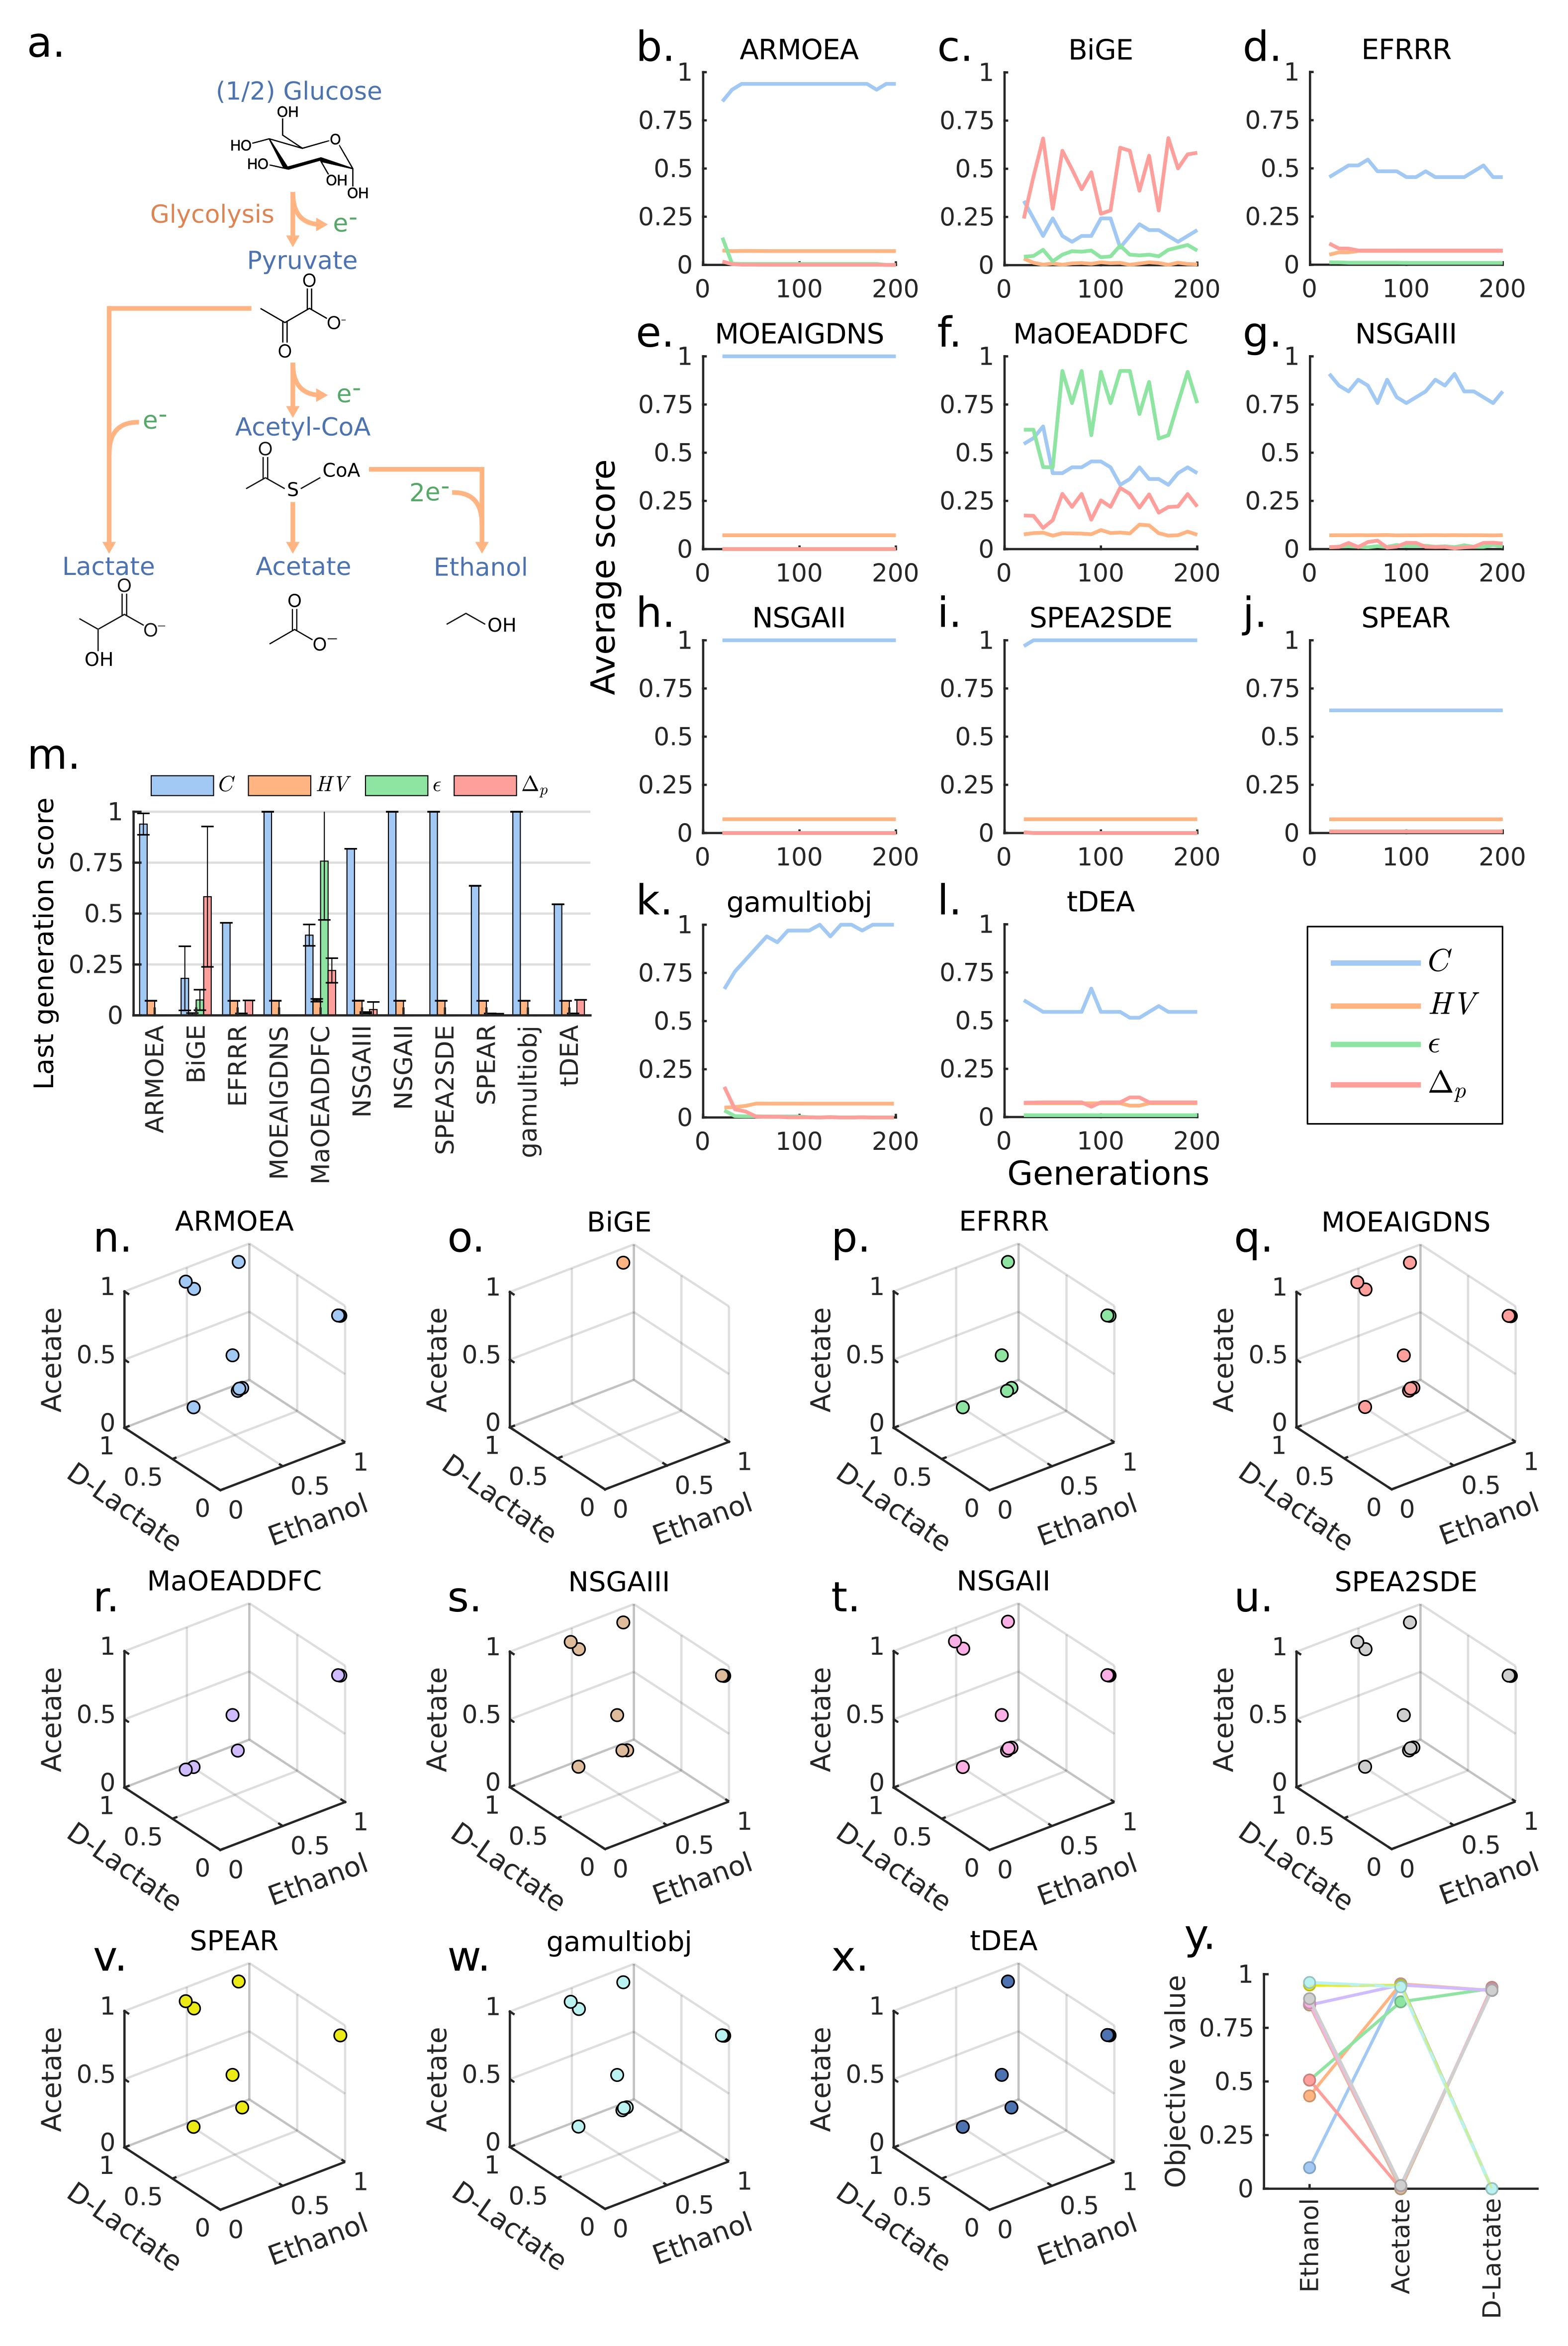
\includegraphics[height=.83\textheight,keepaspectratio]{case1.png}
    %\caption{(Caption next page.)}
    \caption[Comparison of MOEAs for a 3-objectives design problem]{Comparison of MOEAs for a 3-objectives design problem.
	(\textbf{a}) The simplified metabolic pathways for conversion of glucose to the target products. Reducing equivalents are presented with $e^-$.
	(\textbf{b-l}) Generation-dependent performance metrics for various MOEAs.
	(\textbf{m}) Performance metrics for various MOEAs at the last generation.
	(\textbf{n-x}) Pareto fronts of various MOEAs at the last generation. It should be noted that only the first replicate is plotted for clear illustration.
	(\textbf{y}) Reference Pareto front ($\PFs$). Each line represents a solution.}
    \label{fig4:case1}
\end{figure}
%\addtocounter{figure}{-1}
%
%\begin{figure}[t!]
%	\caption{(Previous page.) Comparison of MOEAs for a 3-objectives design problem.
%	(\textbf{a}) The simplified metabolic pathways for conversion of glucose to the target products. Reducing equivalents are presented with $e^-$.
%	(\textbf{b-l}) Generation-dependent performance metrics for various MOEAs.
%	(\textbf{m}) Performance metrics for various MOEAs at the last generation.
%	(\textbf{n-x}) Pareto fronts of various MOEAs at the last generation. It should be noted that only the first replicate is plotted for clear illustration.
%	(\textbf{y}) Reference Pareto front ($\PFs$). Each line represents a solution.}
%\end{figure}

\begin{figure}[H]
    \centering
    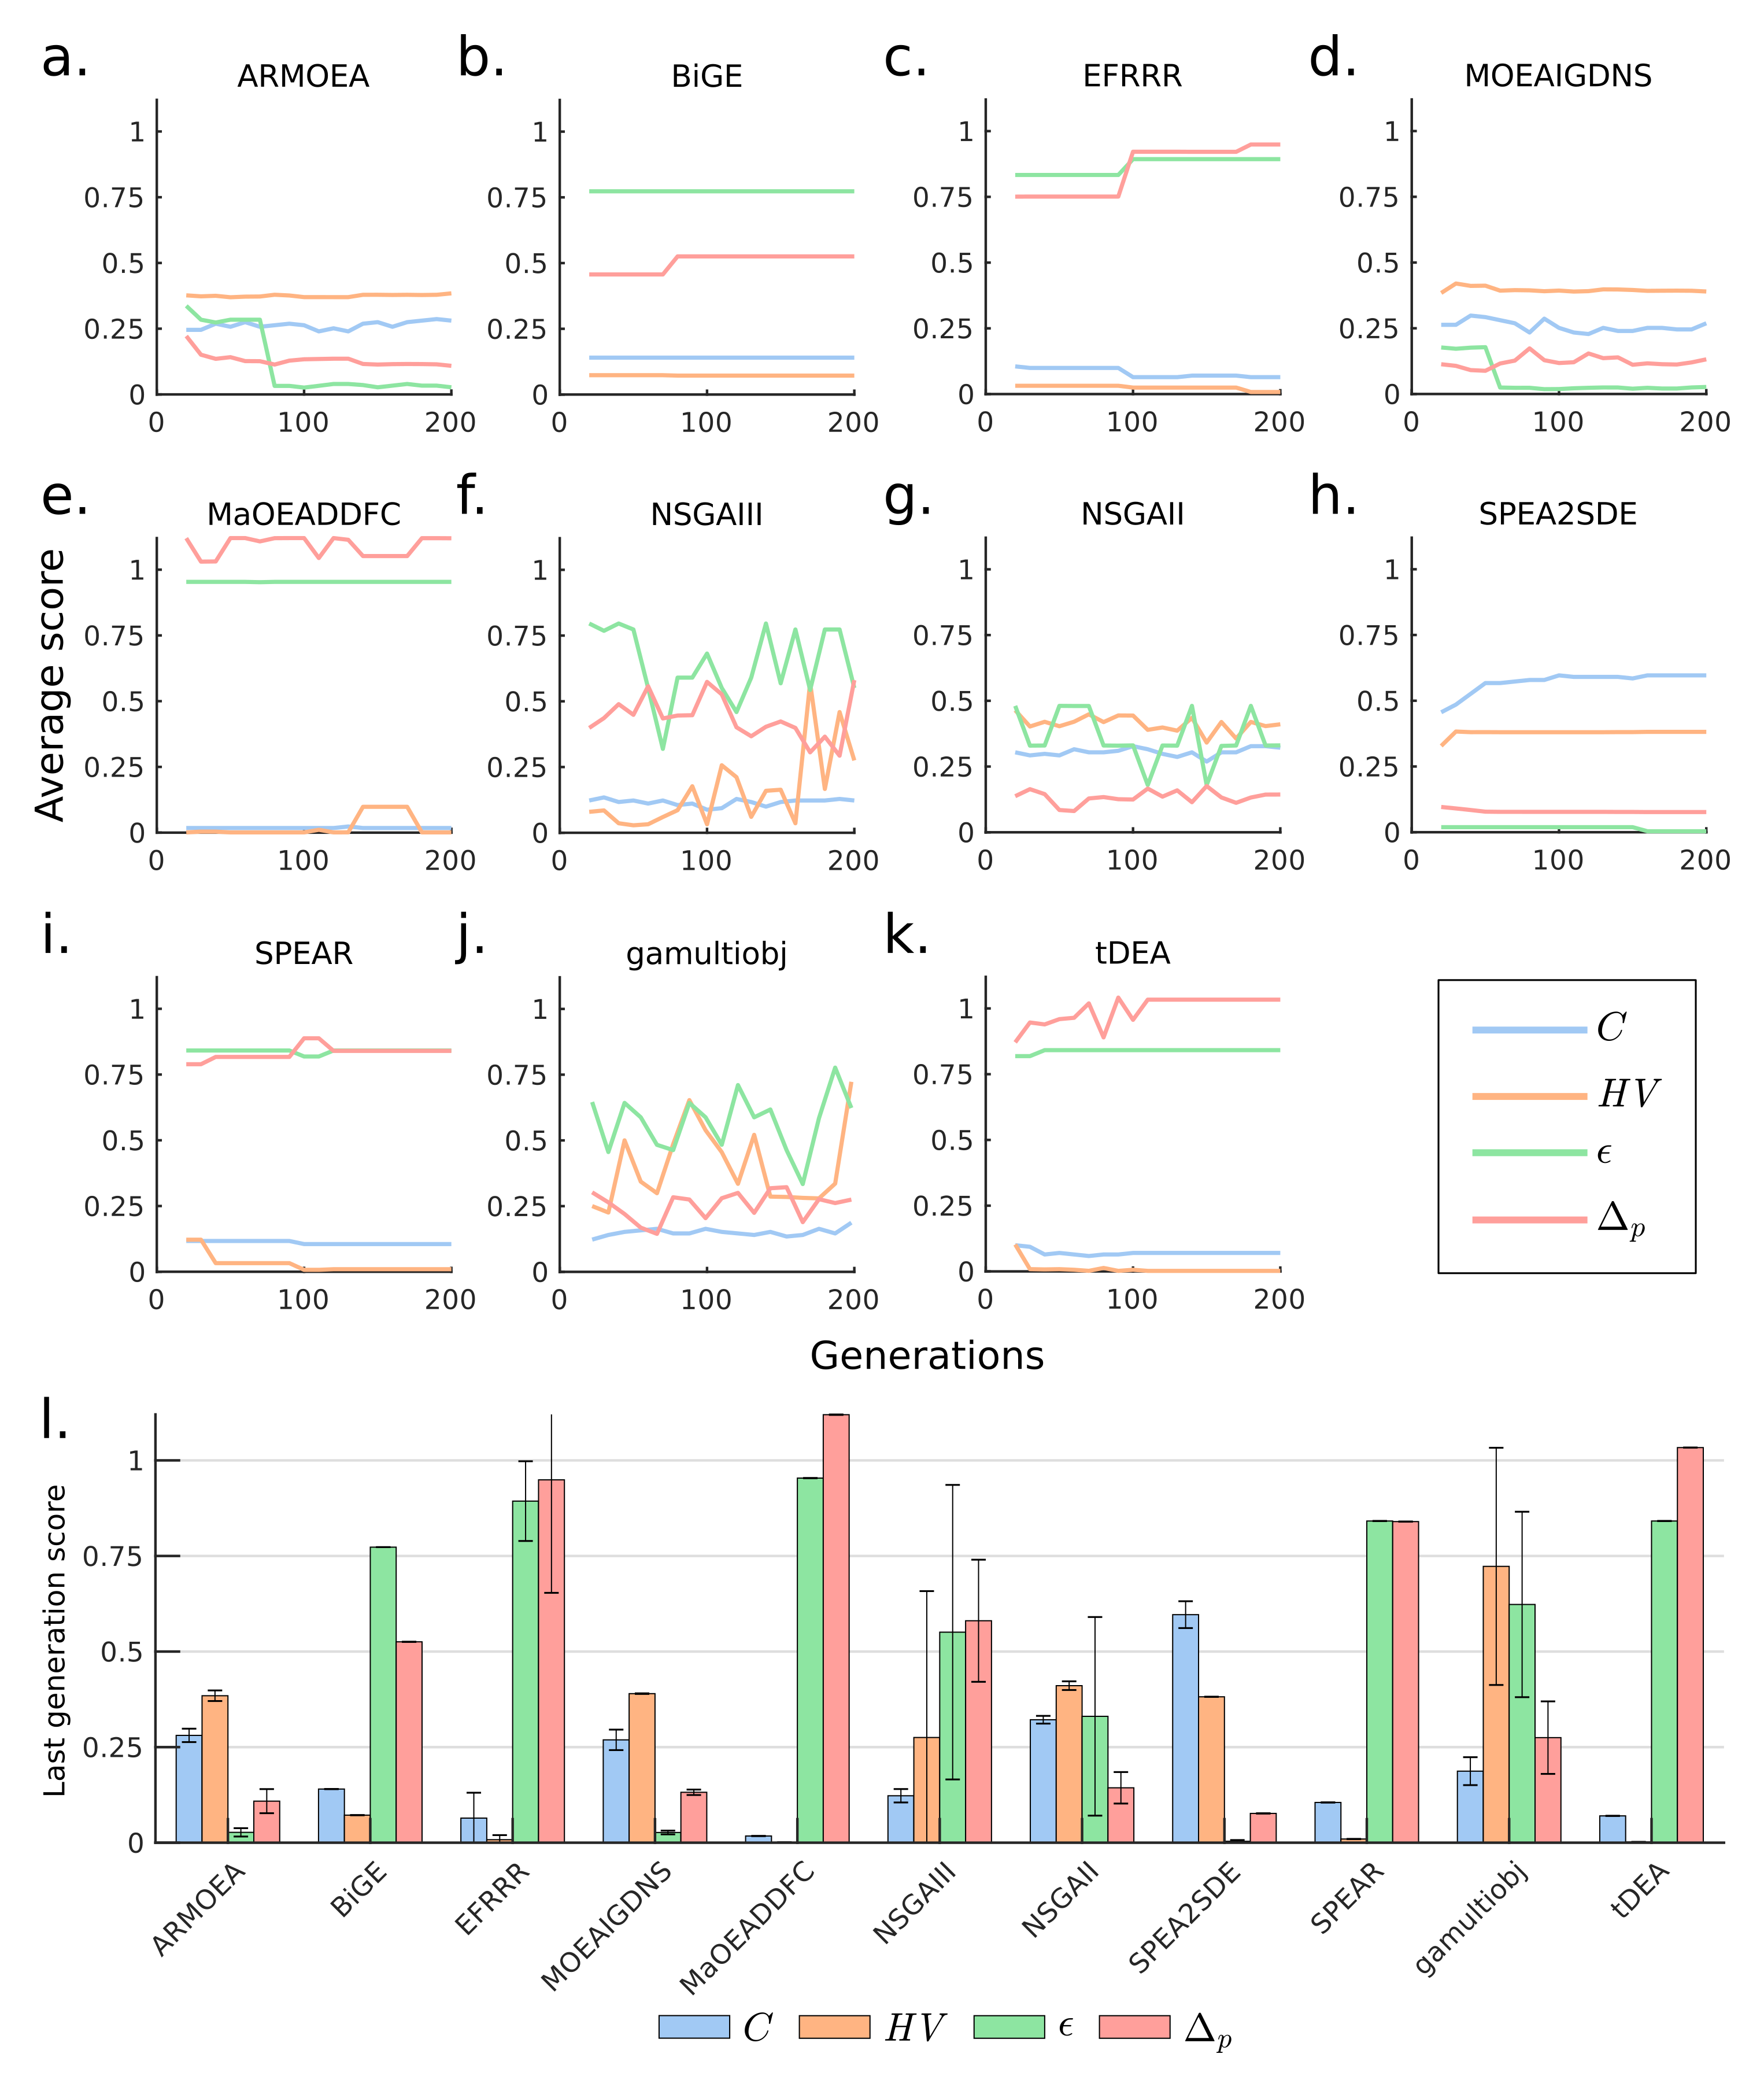
\includegraphics[width=\textwidth,height=\textheight,keepaspectratio]{case2.png}
    \caption[Comparison of MOEAs for a 10-objective design problem]{Comparison of MOEAs for a 10-objective design problem. (\textbf{a-k}) Generation-dependent performance metrics for various MOAEs. (\textbf{l}) Performance metrics for various MOEAs at the last generation.}
\label{fig4:case2}
\end{figure}

\begin{figure}[H]
    \centering
    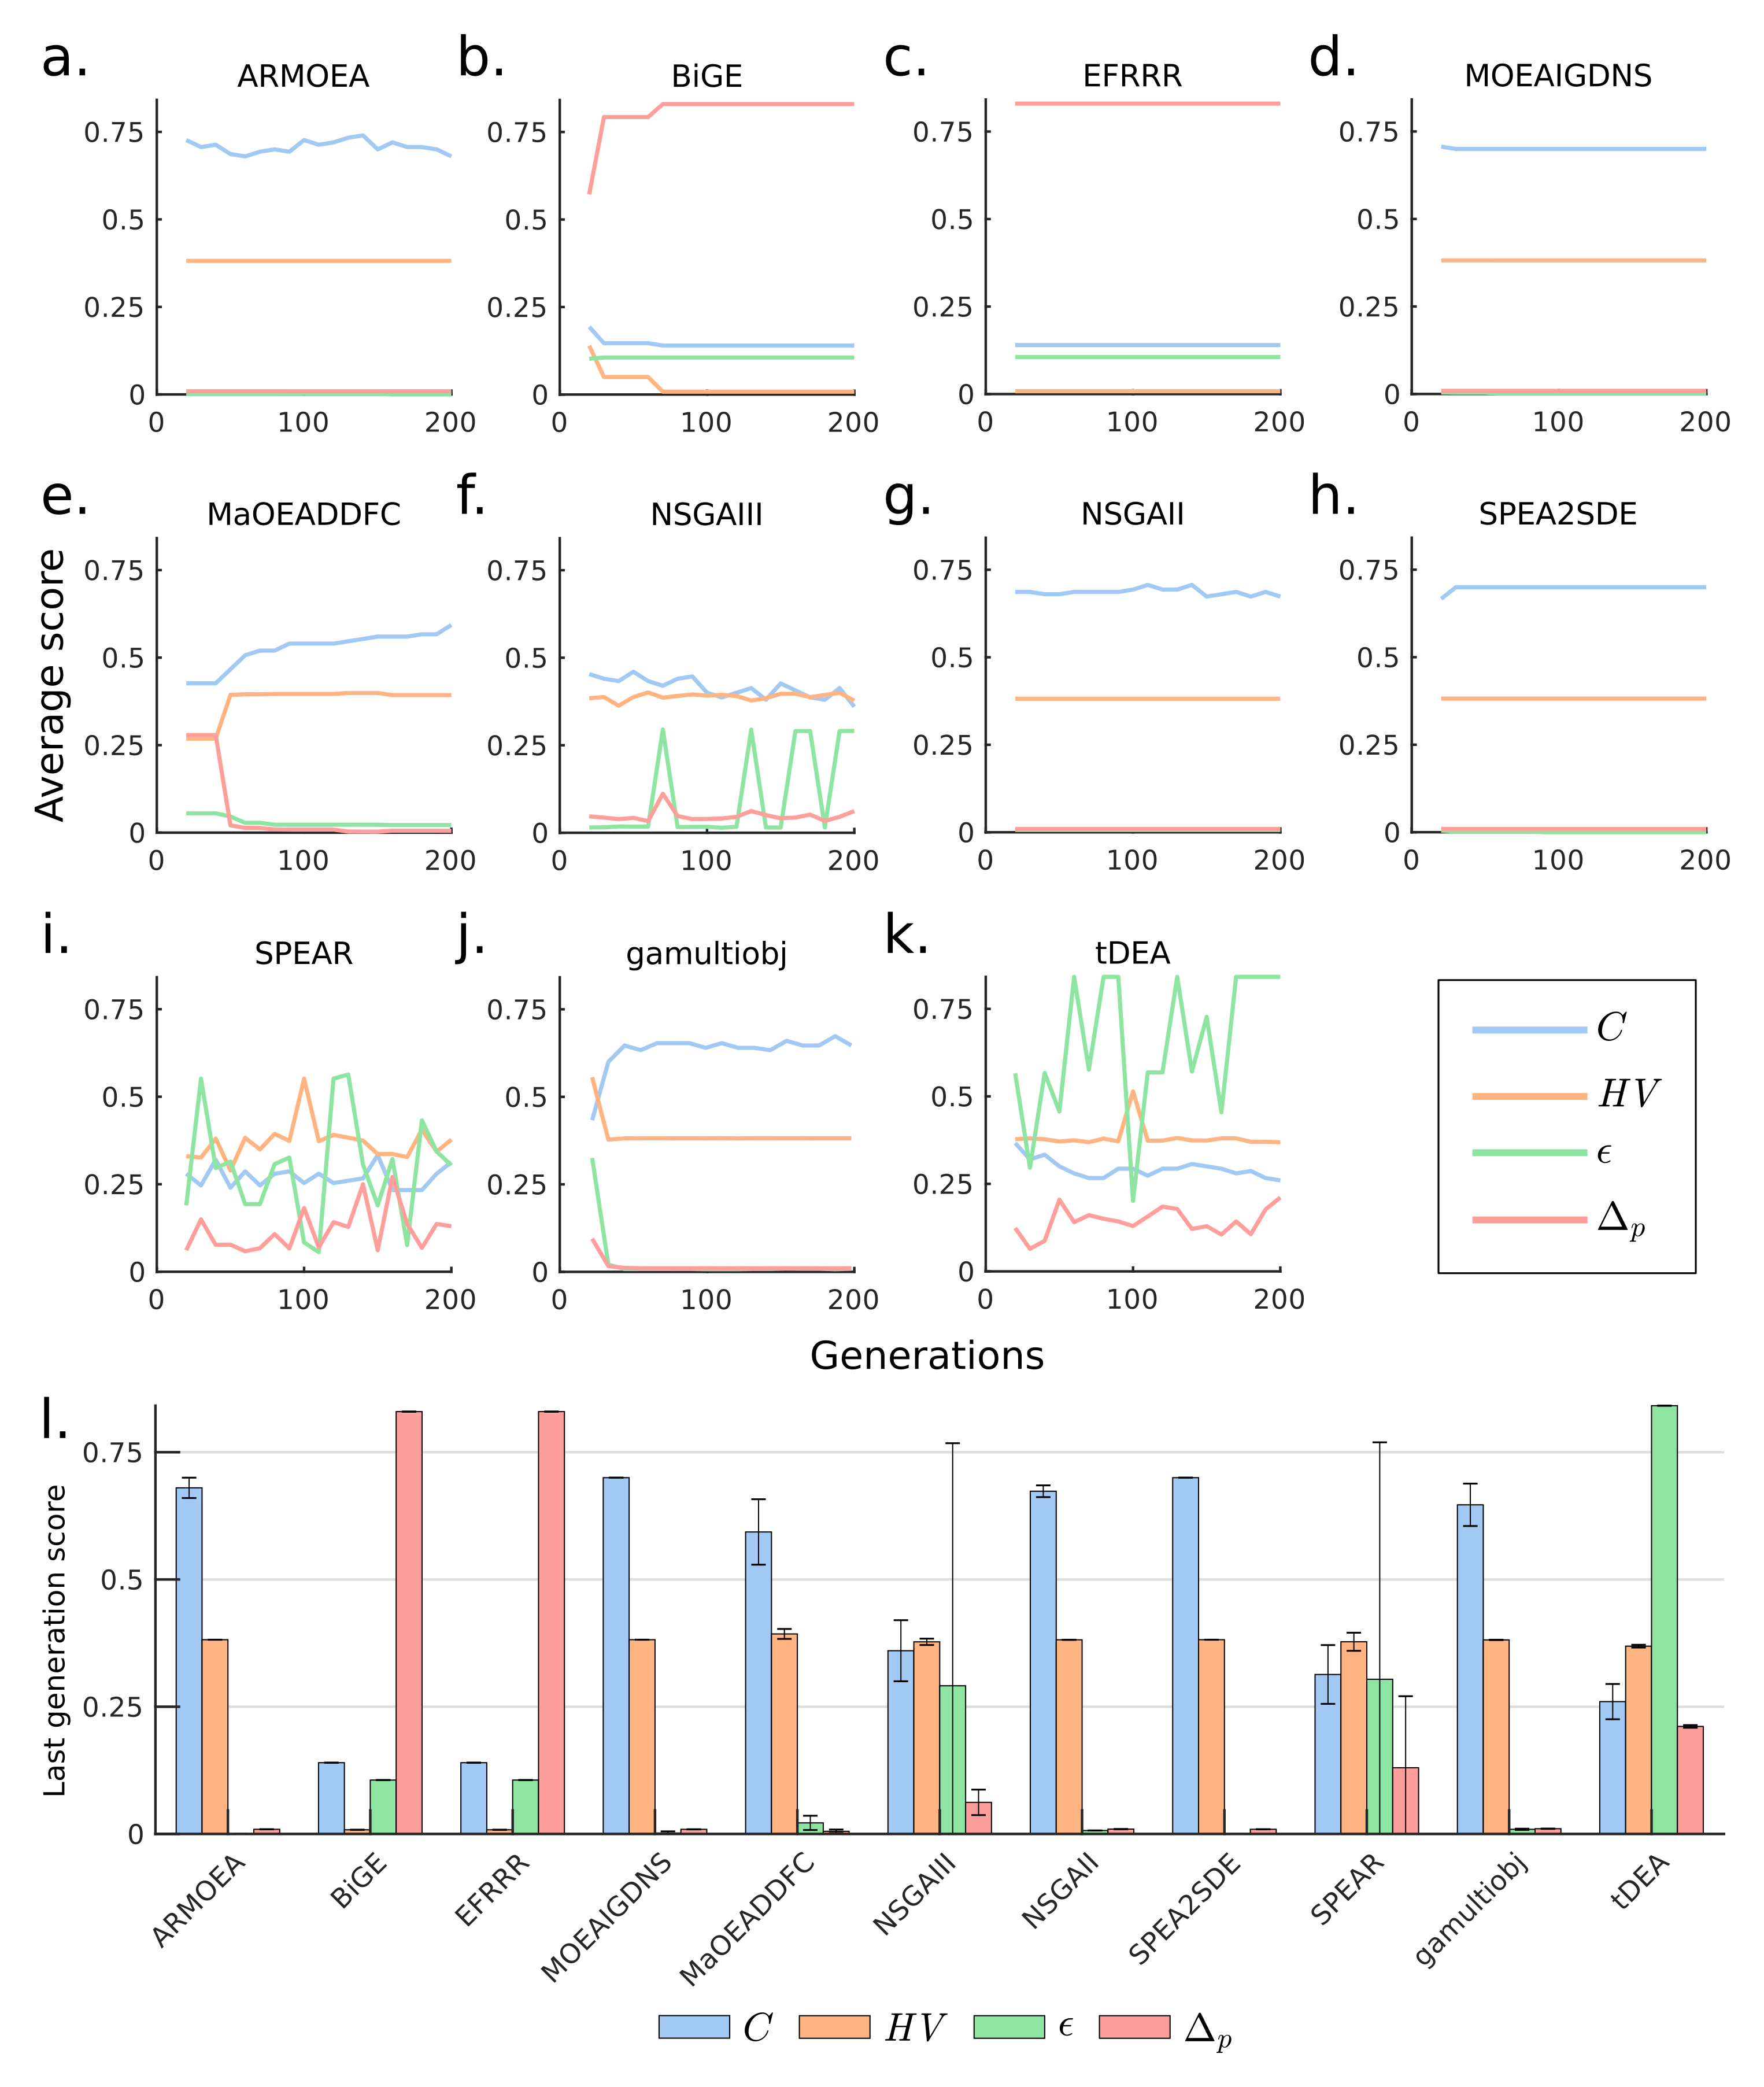
\includegraphics[width=\textwidth,height=\textheight,keepaspectratio]{case3.png}
    \caption[Comparison of MOEAs with increased population sizes]{Comparison of MOEAs for a 10-objectives design problem with larger population sizes
	(\textbf{a-k}) Generation-dependent performance metrics for various MOAEs.	(\textbf{l}) Performance metrics for various MOEAs at the last generation.}
\label{fig4:case3}
\end{figure}

\begin{figure}[H]
    \centering
    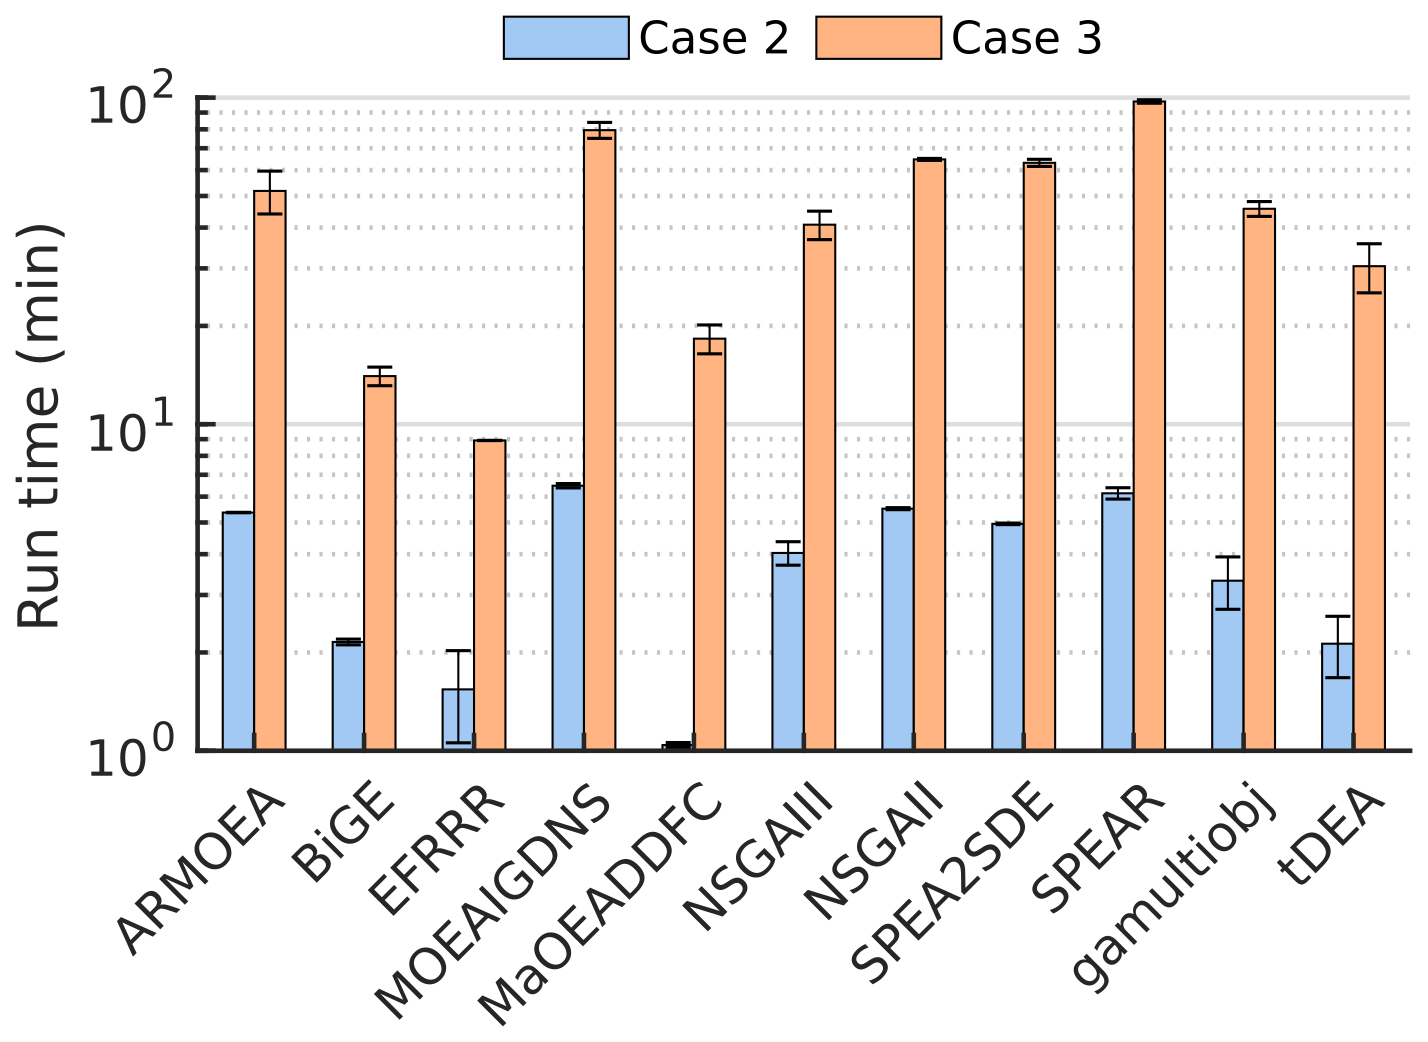
\includegraphics[width=0.45\textwidth,keepaspectratio]{timing.png}
    \caption[Wall-clock run times]{Wall-clock run times for the 10-objectives design problem with population sizes of 100 (Case 2) and 1000 (Case 3).}
\label{fig4:timing}
\end{figure}

%%%%%%%%%%%%%%%%%%%%%%%%%%%%%%%%%%%%%%%%%%

\section{Conclusions}
In this study, we evaluated the performance of several MOEAs to solve the modular cell design problem. SPEA2SDE, the recently developed many-objectives method, was the best performing MOEA for limited population sizes in our study. However, for sufficiently large populations, several algorithms attained the best results, including the well-established NSGAII, which performed better than more recently developed many-objectives MOEAs. We used the most popular performance metrics to compare MOEAs and found that the coverage ($C$) metric is the most valuable indicator. This metric can provide an intuitive quantitative meaning and tends to increase monotonically with the number of generations simulated. In contrast, hypervolume ($\HV$) generally did not differentiate algorithm performance and was misleading in some scenarios where an algorithm generated very few solutions. Overall, these results highlight the need for empirical testing of MOEAs towards specific problems and of the population size as a more important factor in performance than the unique heuristics commonly used by different algorithms.
For the application of modular cell engineering, efficient MOEAs will enable the design of modular cell(s) compatible with many product synthesis modules for large-scale metabolic networks and the identification of more diverse and better solutions that will provide more viable options for practical implementation.

%%%%%%%%%%%%%%%%%%%%%%%%%%%%%%%%%%%%%%%%%%





%%%%%%%%%%%%%%%%%%%%%%%%%%%%%%%%%%%%%%%%%%
%\vspace{6pt}

%%%%%%%%%%%%%%%%%%%%%%%%%%%%%%%%%%%%%%%%%%
%% optional
%\supplementary{The following are available online at \linksupplementary{s1}, Figure S1: title, Table S1: title, Video S1: title.}

% Only for the journal Methods and Protocols:
% If you wish to submit a video article, please do so with any other supplementary material.
% \supplementary{The following are available at \linksupplementary{s1}, Figure S1: title, Table S1: title, Video S1: title. A supporting video article is available at doi: link.}

%%%%%%%%%%%%%%%%%%%%%%%%%%%%%%%%%%%%%%%%%%
%\authorcontributions{conceptualization, S.G. and C.T.; methodology, S.G.; software, S.G.; validation, S.G.; formal analysis, S.G.; investigation, S.G.; resources, S.G.; data curation, S.G.; writing--original draft preparation, S.G.; writing--review and editing, S.G. and C.T.; visualization, S.G. and C.T.; supervision, C.T.; project administration, C.T.; funding acquisition, C.T.}
%\authorcontributions{CTT initiated and supervised the study. SG and CTT designed experiments. SG performed simulation experiments and analyzed data. SG and CTT wrote and approved the manuscript.}

%%%%%%%%%%%%%%%%%%%%%%%%%%%%%%%%%%%%%%%%%%
%\funding{Please add: ``This research received no external funding'' or ``This research was funded by NAME OF FUNDER grant number XXX.'' and  and ``The APC was funded by XXX''. Check carefully that the details given are accurate and use the standard spelling of funding agency names at \url{https://search.crossref.org/funding}, any errors may affect your future funding.}
%\funding{This research was funded by the NSF CAREER Award (NSF\#1553250) and the Center of Bioenergy Innovation (CBI), U.S. Department of Energy Bioenergy Research Center supported by the Office of Biological and Environmental Research in the DOE Office of Science. The views, opinions, and/or findings contained in this article are those of the authors and should not be interpreted as representing the official views or policies, either expressed or implied, of the funding agencies.}

%%%%%%%%%%%%%%%%%%%%%%%%%%%%%%%%%%%%%%%%%%
%\acknowledgments{In this section you can acknowledge any support given which is not covered by the author contribution or funding sections. This may include administrative and technical support, or donations in kind (e.g., materials used for experiments).}

%%%%%%%%%%%%%%%%%%%%%%%%%%%%%%%%%%%%%%%%%%
%\conflictsofinterest{The authors declare no conflict of interest.}
